\documentclass{report}
\usepackage[utf8]{inputenc}
\usepackage{amsmath}
\usepackage{graphicx}

\title{Eksamensnoter - Binary Search Tree}
\author{André Oskar Andersen (wpr684)}
\date{\today}

\begin{document}
\maketitle

\section*{12 Binary Search Trees}
\begin{itemize}
    \item Basic operations on a binary search tree take time proportional to the height of the tree. For a complete binary tree with $n$ nodes, such operations run in $\Theta(\lg n)$ worsst-case time. If the tree is linear chain if $n$nodes, however, the same operation take $\Theta(n)$ worst-case time. If a binary search tree is built randomly, then the expected height is $O(\lg n)$, so that basic dynamic-set operations on such a tree take $\Theta(\lg n)$ time on average
\end{itemize}
\subsection*{12.1 What is a binary search tree?}
\begin{itemize}
    \item A binary search tree is organized in a binary tree. We can represent such a tree by a linked data structure in which each node is an object. In addition to a \textit{key} and satellite data, each node contains attributes \textit{left}, \textit{right}, and $p$ that point to the nodes corresponding to its left child, its right child, and its parent, respectively.
    \item If a child or the parent is missing, the appropriate attribute contains the value \texttt{NIL}. The root node is the only node in the tree whose parent is \texttt{NIL}
    \item The keys in a binary search tree are always stored insuch a way as to satisfy the \textit{binary-search-tree property}:
    \begin{quote}
        Let $x$ be a node in a binary search tree. If $y$ is a node in the left subtree of $x$, then $y.key \leq x.key$. If $y$ is a node in the right subtree of $x$, then $y.key \geq x.key$
    \end{quote}
\end{itemize}
\subsection*{12.2 Querying a binary search tree}
\begin{itemize}
    \item Besides the \texttt{SEARCH} oepration, binary search trees can support such quieries as \texttt{MINIMUM}, \texttt{MAXIMUm}, \texttt{SUCCESSOR}, and \texttt{PREDECESSOR}. Each one has a runtime of $O(h)$ on a binary search tree of height $h$.
\end{itemize}
\subsection*{12.3 Insertion and deletion}
\textbf{Insertion}
\begin{itemize}
    \item Like the other primitive operations on search trees, the procedure \texttt{TREE-INSERT} runs in $O(h)$ time on a tree of height $h$
\end{itemize}
\textbf{Deletion}
\begin{itemize}
    \item The procedure for deleting a given node $z$ from a binary search tree $T$ takes as arguments pointers to $T$ and $z$:
    \begin{itemize}
        \item If $z$ has no left child, then we replace $z$ by its right child, which may or may not be \texttt{NIL}.
        \item If $z$ has just one child, which is its left child, then we replace $z$ by its left child
        \item Otherwise, $z$ has both a left and a right child. We find $z$'s sucessor $y$ (smallest number which is greater than $z$), which lies in $z$'s right subtree and has no left child. We want to splice $y$ out of its current location and have it replace $z$ in the tree:
        \begin{itemize}
            \item If $y$ is $z$'s right child, then we replace $z$ by $y$, leaving $y$'s right child alone
            \item Otherwise, $y$ lies within $z$'s right subtree but is not $z$'s right child. In this case, we first replace $y$ bt its own right child, and then we replace $z$ by $y$
        \end{itemize}
    \end{itemize}
    \item \texttt{TREE-DELETE} runs in $O(h)$ time on a tree of height $h$
\end{itemize}

\section*{13 Red-Black Trees}
\begin{itemize}
    \item Red-black trees are one of many search-tree schemes that are "balanced" in order to guarantee that basic dynamic-set operations take $O(\lg n)$ time in the worst case
\end{itemize}
\subsection*{13.1 Properties of red-black trees}
\begin{itemize}
    \item A \textit{red-black tree} is a binary search tree with one extra bit of storage per node: its \textit{color}, which can be either RED of BLACK.
    \item A red-black tree is a binary tree that satisfies the following \textit{red-black properties}:
    \begin{itemize}
        \item Every node is either red or black
        \item The root is black
        \item Every leaf (\texttt{NIL}) is blackIf a node is red, then bots its children are blackFor each node, all simple paths from the node to descendant leaves contain the same number of black nodes
        \item If a node is red, then both its children are black
        \item For each node, all simple paths from the node to descendant leaves contain the same number of black nodes
    \end{itemize}
    \item We call the number of black nodes on any simple path from, but not including, a node $x$ down to a leaf the \textit{black-height} of the node, denoted $bh(x)$. We define the black-height of a red-black tree to be the height of its root
\end{itemize}
\textbf{Lemma 13.1}
\begin{itemize}
    \item A red-black tree with $n$ internal nodes has height at most $2 \lg(n + 1)$
    \item As an immediate consequence of this lemma, we can implement the dynamic-set operations \texttt{SEARCH}, \texttt{MINIMUM}, \texttt{MAXIMUM}, \texttt{SUCCESSOR}, and \texttt{PREDECESSOR} in $O(\lg n)$, since eahc can run in $O(h)$ time on a binary search tree of height \textit{h} and any red-black tree on $n$ nodes is a binary search tree with height $O(\lg n)$ 
\end{itemize}
\subsection*{13.2 Rotations}
\begin{center}
    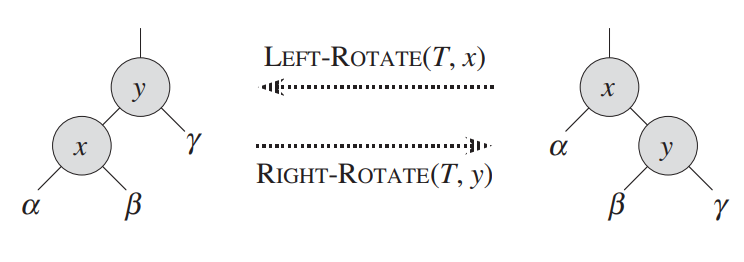
\includegraphics[height = 3 cm]{../entities/fig_13_2.png}
\end{center}
\begin{itemize}
    \item The search-tree operations \texttt{TREE-INSERT} and \texttt{TREE-DELETE}, when run on a red-black tree with $n$ keys, take $O(\lg n)$ time. Because they modify the tree, the result may violate the red-black properties. To restore these properties, we must change the colors of some of the nodes in the tree and also cahnge the pointer structure
    \item We change the pointer structure through \textit{rotation}, which is a local operation in a search tree that preserves the binary-search-tree property. There are two kinds of rotations: left ortations and right rotations.
\end{itemize}
\subsection*{13.3 Insertion}
\begin{itemize}
    \item We can insert a node into an $n$-node red-black tree in $O(\lg n)$ time.
\end{itemize}
\subsection*{13.4 Deletion}
\begin{itemize}
    \item Deletion of a node takes time $O(\lg n)$
\end{itemize}
\section*{33 Computational Geometry}
\subsection*{33.1 Line-segment properties}
\begin{itemize}
    \item A \textit{convex combination} of two distinct points $p_1 = (x_1, y_1)$ and $p_2 = (x_2, y_2)$ is any point $p_3 = (x_3, y_3)$ such that for some $\alpha$ in the range $0 \leq \alpha \leq 1$, we have $x_3 = \alpha x_1 + (1 - \alpha)x_2$ and $y_3 = \alpha y_1 + (1 - \alpha) y_2$. We also write that $p_3 = \alpha p_1 + (1 - \alpha) p_2$. Intuitively, $p_3$ is any point that is on the line passing through $p_1$ and $p_2$ and is on or between $p_1$ and $p_2$ on the line.
    \item Given two distinct points $p_1$ and $p_2$, the \textit{line swegment} $\bar{p_1p_2}$ is the set of convex combinations of $p_1$ and $p_2$
    \item We call $p_1$ and $p_2$ the \textit{endpoints} of segment $\bar{p_1p_2}$.
    \item Sometimes the ordering of $p_1$ and $p_2$ matters, and we speak of the \textit{directed segment} $\overrightarrow{p_1p_2}$
    \item If $p_1$is the origin, then we can treat the directed segment $\overrightarrow{p_1p_2}$ as the vector $p_2$
\end{itemize}
\textbf{Cross products}
\begin{itemize}
    \item If $p_1 \times p_2$ is positive, then $p_1$ is clockwise from $p_2$ with respect to the origin. If the cross product is negative, then $p_1$ is counterclockwise from $p_2$. If the cross product is 0, then the vectors are \textit{colinear}, pointing in either the same or opposite directions
\end{itemize}
\end{document}